\section{Nodes of crosstalk between \tgfbsf\ and Wnt}
\label{pathways:wntTgfb:mechanism}


In this dissertation I am interested in understanding the inter-pathway
crosstalk between \tgfbsf\ and Wnt. As discussed in \ar{introduction:encoding},
one of the most problematic aspects of studying cell signaling
is the determination of which input signals a cell cares about
and into what intracellular property that information is encoded.
As this chapter has so far detailed, the field consensus for both
\tgfbsf\ and Wnt is that it is the concentration of the ligands
that carries the information that cells care about
(these are morphogenic signals) and this
information is encoded into nuclear concentrations of canonical
transcription factors.


Further, the literature reviewed in the previous section
strongly suggest that the \tgfbsf\ and Wnt
pathways have many opportunities for crosstalk, especially in the
mammalian gut. With established input/output relationships
in hand, and reason to suspect that the pathways in question modulate one
another, we can begin to ask how these pathways integrate information.
This section provides a review of the signaling nodes at which
inter-pathway crosstalk is thought to occur (see the graphical
summary in \ar{fig:pathways:xtalk}).




  \begin{figure}[!bt]
  \centering
  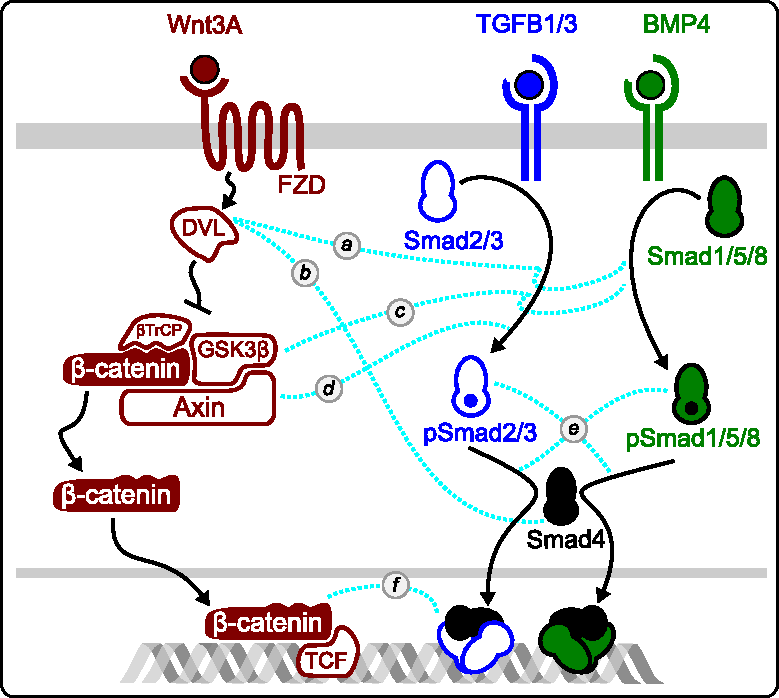
\includegraphics[width=4in]{FIGS/pathways/tgfb_wnt_xtalk.pdf}
  {\singlespacing 
  \caption[Overview of Wnt and \tgfbsf\ pathway crosstalk]
        { Overview
          of Wnt and \tgfbsf\ pathway crosstalk. 
          This dissertation focuses on canonical Wnt, BMP, and \tgf\, as mediated by Wnt3A,
          BMP4, and \tgf 1/3. Dashed lines indicate
          literature-established
          links between pathways. References:
          \textit{a}\cite{Warner2003,Warner2005a,Liu2006};
          \textit{b}\cite{Mamidi2012};
          \textit{c}\cite{Fuentealba2007,Guo2008};
          \textit{d}\cite{Furuhashi2001,Guo2008,Liu2006b};
          \textit{e}\cite{Candia1997};
          \textit{f}\cite{Zeng2008}.}
  \label{fig:pathways:xtalk}}
  \end{figure}




\subsection{Smad and DVL}
\label{pathways:wntTgfb:dvl}

The DVL proteins, being key post-receptor mediators
of both canonical and non-canonical signaling, occupy
an important position for potential crosstalk with
the \tgfbsf\ pathway. Interactions of DVL with
the MH2 domain of Smads were first identified in a yeast two-hybrid
screen \cite{Warner2003}. The same group and others confirmed
the possibility of such interactions in mammalian cells using
co-immunoprecipitation (co-IP) after overexpression of Smads, with the
conclusion that all three DVLs could bind to most of the
Smads (\ar{fig:pathways:xtalk}a) \cite{Warner2003,Warner2005a,Liu2006}. The Smad-DVL
interaction was also shown for non-canonical Wnt signaling,
with a downstream mediator of Wnt5A, PAR1B, precipitating with both
Smad and DVL (\ar{fig:pathways:xtalk}b) \cite{Mamidi2012}.


While co-IP of overexpressed proteins shows the possibility of interaction,
they neither guarantee that it occurs under normal conditions
nor imply that the interaction has a functional outcome.
In some of the studies cited above, attempts were made
to demonstrate functional consequences of Smad-DVL interaction.
This was done by treating cells with ligands for one or both
pathways after ablation or overexpression of other signaling components.
Using this approach, it was found that BMP2 treatment
could increase complexed DVL1/Smad1, while
Wnt3A-conditioned media had the opposite effect \cite{Liu2006},
suggesting that pathway interactions are sensitive to signaling activity.
Additionally, RNAi of
all three DVLs, PAR1B, or ROR2 can attenuate TGFB signaling, while
overexpression of DVL3 or FZD2 can enhance it
\cite{Mamidi2012,Miyoshi2012}.
The authors of these studies interpreted the data to mean that the
\tgfbsf\ pathway is directly modulated by the Wnt pathways during
signal transduction, though the mechanisms are unclear and seemingly
complex. Importantly, the observed cross-pathway modulation seemed to be mediated
by interactions between DVL and Smad.


A functional consequence of TGFB and non-canonical Wnt5A
integration was recently reported in the context of wounded
colonic epithelium \cite{Miyoshi2012}. In that study, the
authors found that mice lacking Wnt5A were less able to repair
colonic epithelial lesions, seemingly due to an inability of
progenitor cells to differentiate in the wound. Given the use of
\tgfbsf\ pathways in gut stem cell differentiation, it is perhaps
unsurprising that the authors could link a \tgf\ signaling
deficiency to this Wnt5A phenotype. Specifically, they
found that treatment of \textit{ex vivo} colonic
crypts with high concentrations of Wnt5A yielded downstream
\tgf\ responses. The mechanisms for this were not clear, except
for a dependence on the TGFBR2 and ROR2 receptors, but are
consistent with DVL-mediated interactions. Importantly, my
own work is suggestive that this Wnt5A/\tgf\ connection is due to an artifact
(\ar{insulation:system}).


\subsection{Smad and Axin}
\label{pathways:wntTgfb:axin}


Axin, being a large protein that is central
to canonical Wnt signaling, is another good candidate
for interactions with \tgfbsf\ components
(\ar{fig:pathways:xtalk}d). Indeed,
in a co-overexpression assay of Axin and Smad3,
the two proteins were found to co-IP. This interaction was
dependent upon a region of Axin between the \bcat\ and
DVL binding domains, though how binding to this site
might affect Wnt signaling is unclear.
Further, \tgf\ responsiveness was
increased when Axin was overexpressed \cite{Furuhashi2001}.
This was interpreted to mean that Axin can stabilize
Smad activity, either by preventing Smad degradation or
by blocking some other form of Smad interference. 


Two additional studies looked into the consequences
of Smad-Axin interactions, but with contradictory results.
In one case, Axin was found
to bind to an iSmad (Smad7) and to mediate degradation
of that Smad by Arkadia, an E3 ubiquitin ligase. As
a consequence, overexpression of both Axin and Arkadia
led to enhanced TGFB signaling \cite{Liu2006b}. While
the outcome is the same as that described above, the
mechanism is essentially the opposite. In
a different study, Axin was again found to destabilize
a Smad, but this time an rSmad via \gsk\
instead of an iSmad via \ubn. As a result, TGFB signaling was instead
attenuated by increased Axin, and
Axin depletion by RNAi amplified TGFB signaling \cite{Guo2008}.


How can we make sense of the studies of Axin-Smad
interaction, that are all mutually incompatible? It is important
here to recall that basal Axin levels in cells are extremely
low \cite{Lee2003}. Because this protein acts as a scaffold,
its overexpression can have a few obvious non-physiological
effects. The first is that Axin is a big protein, with many
binding surfaces, and so the observed Smad-Axin interactions
may be due to what would normally be extremely rare binding
events. The other is that while Smad and Axin may interact,
overexpression of the scaffold causes interactions between Smad and other
Axin-bound proteins to become at first enhanced and then diluted
as the amount of Axin increases. All of the cited studies use
Axin overexpression, and so the apparent contradictions between them
may be due to either of these phenomena.



\subsubsection{Smad and \gsk}
\label{pathways:wntTgfb:gsk}

\gsk, which primes \bcat\ for \ubn, is able to phosphorylate a large
fraction of the proteome. Recently, this was found include the bSmads
(experimentally) and the tSmads (based on computational prediction).
The Smads have a canonical \gsk\ recognition sequence in the linker region
between the functional MH1 and MH2 domains. Phosphorylation of these sites
in bSmads was found to be \gsk-dependent and could be 
down-regulated by Wnt3A treatment (\ar{fig:pathways:xtalk}c). Importantly, the study
found that total Smad levels were not affected by Wnt treatment, but
that the active phospho-state did show measurable decreases \cite{Fuentealba2007}.
This data was therefore interpreted to mean that \gsk\ could modulate
the long-term duration of Smad activity.


\subsubsection{Smad and \bcat}
\label{pathways:wntTgfb:bcat}


Finally, we turn to interactions with the final effector of
the Wnt pathway, \bcat\ (\ar{fig:pathways:xtalk}f).
Like Axin, the large size of \bcat\ provides
many potential binding interfaces. Additionally, its role as the bottleneck
of all canonical Wnt signaling makes it a good candidate for
cross-pathway interaction. Even so, evidence for interactions between
Smad and \bcat\ are quite limited. There is some evidence that
\fly\ MAD and Armadillo (Smad and \bcat\ orthologs) compete with one another
for binding to TCF, such
that DPP (the BMP2/4 ortholog) can cause a downstream block of \bcat\ transcriptional output
\cite{Zeng2008}. Similarly, though with different functional consequences, in mammals
an iSmad (Smad7) can co-IP with \bcat\ and overexpressed TCF/Lef \cite{Edlund2005}.
It is therefore unclear whether a Smad/\bcat\ interaction is important to signaling
through either pathway.


  
\subsubsection{Transcriptional crosstalk}
\label{pathways:wntTgfb:transcription}


The nodes of putative crosstalk described above occur prior to transcription
factor entry into the nucleus. I therefore classify these as nodes of 
``signaling crosstalk.'' What about at the level of transcription,
after the nucleus has received the transcription factor output of each signaling pathway?
Our knowledge of \tgfbsf/Wnt crosstalk is almost entirely due to studies
at this level of interaction, however studies that look at both pathways
simultaneously are rare. Instead, transcriptional crosstalk is often inferred
by studies finding that activity of one pathway
modulates transcriptional output commonly associated with the other.


A few direct crosstalk studies have been performed, though their results
are not easily comparable.
In the case of TGFB and Wnt, activation of both pathways was found to
increase output of a Wnt transcriptional reporter. The lack of
Smad-response elements in this promoter suggested that
the co-activation was due to an interaction occurring prior to promoter
binding \cite{Warner2005,Lei2004}. Microarrays
from similar co-treatment experiments showed that a set of genes
were regulated differently in the context of both inputs than with either
input alone, though no obvious patterns were found (e.g. genes that
were increased by Wnt or TGFB were not necessarily further increased by both)
\cite{Warner2011,Labbe2007}.


Transcriptional crosstalk is most frequently inferred by the presence
of consensus binding motifs for \bcat/TCF and the Smads within the
same target gene promoter. In this way, 
instances of direct transcriptional co-regulation by TGFB/Wnt
have been found in several systems 
\cite{Hussein2003,Zhou2012,Labbe2000,Rodriguez-Carballo2011}.
For the focal case of the gut in this section, the
co-regulation of the Myc promoter by these two sets of transcription factors
is of obvious relevance \cite{Hu2005} .

